\chapter{Reinforcement learning}
\label{cha:reinforcement_learning}
%\cite{Sutton1998ReinforcementIntroduction.}.
In reinforcement learning, one tries to find which action to take in a certain state of the environment in order to maximize a possibly delayed numerical reward.\\
For chapters \ref{sub:rl:basics} to \ref{sec:rl:bootstrapping} and \ref{sub:rl:gfa}, we will closely follow the explanation by \cite{Sutton1998ReinforcementIntroduction}.

\section{Basics}
\label{sub:rl:basics}
Reinforcement learning problems can be formulated in the form of a Markov Decision Process (MDP).
This is four-tuple $(\mathcal{S}, \mathcal{A}, \mathcal{P}, \mathcal{R})$. $\mathcal{S}$ is the state space and contains all the possible states of the environment. The action space, $\mathcal{A}$, denotes all the possible actions that the agent can take in the environment. $\mathcal{P}: \mathcal{S} \times \mathcal{A} \to \mathcal{S}$ is the transition function and defines the probabilities for being in next state given a state and an action.
$\mathcal{R}: \mathcal{S} \times \mathcal{A} \to \mathcal{R}$ gives probabilities for rewards when taking an action in a certain state.
A transition is then a tuple of a state, an action taken at that state, the received reward by taking that action (determined using $\mathcal{R}$) and the next state (determined using $\mathcal{P}$): $(s_t,a_t,r_t,s_{t+1})$. A sequence of transitions is called a trajectory.

A reinforcement learning algorithm does not know on beforehand which actions are optimal. As such, this must be discovered by trial-and-error. Subsequently, it can change its policy to increase the achieved rewards. This policy, denoted by $\pi$, defines for each state and action a probability $\pi(s,a)$, which denotes the probability of taking action $a$ when in state $s$: $\pi_t(s,a) = P(a_t = a \vert s_t = s)$. Note that exactly one action has to be taken in a state and that the action probabilities for one state sum to $1$: $\sum_{a\in \mathcal{A}}\pi_t(s,a)=1$.\\
Because feedback in the form of numerical rewards may not be immediate, a reinforcement learning algorithm must be able to backtrack which actions in certain situation lead to the reward that the reinforcement learning algorithm received.\\

Reinforcement learning algorithms often use a state-value function $V(s)$. This function says how good it is to be in a certain state $s$ by stating the expected return in the future starting from state $s$, where the return is the discounted rewards. This expected value when starting in state $s$ and following a specific policy $\pi$ is denoted as $V^\pi(s)$:
\begin{equation}
\label{eq:vpolicy}
V^\pi(s) = \ex_\pi\{R_t \vert s_t=s\}=\ex_\pi\big \{ \sum_{k=0}^{\infty}\gamma^k r_{t+k+1} \vert s_t=s\big \}
\end{equation}
Where $\gamma$ is a discount applied over time to past rewards. The optimal policy $\pi$ is the one that leads to the highest $V^\pi(s)$ for all $s \in \mathcal{S}$. The resulting state-value function is $V^*(s) = \max_\pi V^\pi(s)$ for all $s \in \mathcal{S}$.

% Like for states, it is also possible to use the value of an action $Q_t(a)$ at time step $t$. Which can be calculated by averaging the rewards obtained by applying action $a$ to time step $t$:
% \begin{equation}
% Q_t(a) = \frac{r_1 + r_2 + \dots + r_{k_a}}{k_a}
% \end{equation}

It is also possible to define a value for taking an action in a certain state, which is the action-value function $Q(s,a)$. $Q^\pi(s,a)$ is the expected return after taking action $a$ in state $s$:
\begin{equation}
Q^\pi(s,a) = \ex_\pi\{R_t|s_t=s,a_t=a\}=\ex_\pi\big \{ \sum_{k=0}^{\infty}\gamma^k r_{t+k+1} | s_t=s,a_t=a\big \}
\end{equation}
Similarly as with $V^*(s)$, $Q^*(s,a)$ is the action-value function we have when applying the optimal policy.\\
Actions can be selected by for example $\epsilon$-greedy or softmax. In $\epsilon$-greedy action selection, the action with the highest $Q(s,a)$ is selected with probability $1-\epsilon$ and a random action otherwise.\\
Softmax chooses an action $a$ when in state $s$ with the following probability:
\begin{equation}
p(s,a) = \frac{e^{Q(s,a)/\tau}}{\sum_{b=1}^n e^{Q(s,b)/\tau}}
\end{equation}
Where $\tau$ is called the temperature and controls the balance between exploration and exploitation. For low values, the best actions are highly probable. For $\tau \to 1$, the probability distribution becomes uniform.\\

%Chapter 4
\section{Dynamic programming}
\label{sub:rldp}
In Dynamic programming, the whole model of the problem is known. A such, we have the complete probability distribution of all the possible transitions. For example, to evaluate a policy $\pi$:
\begin{align}
\begin{split}
V^{\pi}(s) &= \ex_{\pi} \{r_{t+1} + \gamma r_{t+2} + \gamma^2r_{t+3}+\dots \mid s_t=s\}\\
&= \ex_{\pi} \{r_{t+1} + \gamma V^{\pi}(s_{t+1}) \mid s_t=s\}\\
&= \sum_a \pi(s,a) \sum_{s'} \mathcal{P}^a_{ss'} [\mathcal{R}^a_{ss'} + \gamma V^{\pi}(s')]
\end{split}
\end{align}
Here, $\pi(s,a)$ is the probability of taking action $a$ in state $s$. This $V^{\pi}(s)$ can be computed using iterative updates for every $s$:
\begin{align}
\begin{split}
V_{k+1}(s) &= \ex_{\pi}\{r_{t+1} + \gamma V_k(s_{t+1}) \vert s_t=s\}\\
&= \sum_a \pi(s,a) \sum_{s'}\mathcal{P}^a_{ss'} [\mathcal{R}^a_{ss'} + \gamma V_k(s')]
\end{split}
\end{align}
This iteration stops when this state-value function has converged. As can be seen, every possible next states is used in the computation instead of just a sample. Because of this, this kind of updates is called a full backup.
Note that we use an estimate of the value function to update the estimate itself. This is called bootstrapping.\\
The optimal state-value function $V^*(s)$ and state-action-value function $Q^*(s,a)$ can be calculated using the following formulas:
\begin{gather}
\begin{split}
V^{*}(s) &= \max_a E\{r_{t+1} + \gamma V^{*}(s_{t+1}) \vert s_t = s, a_t = a\}\\
&= \max_a \sum_{s'} \mathcal{P}^a_{ss'} [\mathcal{R}^a_{ss'}+\gamma V^{*}(s')]
\end{split}\\
\begin{split}
Q^{*}(s,a) &= E\{r_{t+1} + \gamma \max_{a'} Q^{*}(s_{t+1},a') \vert s_t=s, a_t=a\}\\
&= \sum_{s'} \mathcal{P}^a_{ss'} [\mathcal{R}^a_{ss'}+\gamma \max_{a'} Q^{*}(s',a')]
\end{split}
\end{gather}

\section{Monte Carlo and Temporal-Difference}
\label{sub:rl_mctd}
Unlike dynamic programming, model-free methods don't require complete knowledge of the environment. Instead, only sample transitions are needed. This way, 2 problems with dynamic programming can be solved. First, the model may be large, which makes it infeasible to use for computing for example an optimal policy. Second, in real world problems, a complete model of the problem may not be available. It may for example be unknown what is the probability of ending in a certain state when taking a certain action from a start state.\\
Monte Carlo methods collect sample returns and average them in order to approximate a value function. The incremental implementation for approximating $V$ is as follows:
\begin{equation}
V(s_t) \leftarrow V(s_t) + \alpha\big[R_t - V(s_t)\big]
\end{equation}
Where $R_t$ is the actual return of an action and $\alpha$ is a constant step-size parameter. As was shown in equation \ref{eq:vpolicy}, to compute $R_t$ we need all the future rewards until the end of the episode.\\
Temporal-Difference (TD) learning tries to solve this by bootstrapping techniques like in dynamic programming. To do this, in the update we replace the full return using the observed reward and the estimate of the value of the next state. This is known as TD(0):
\begin{equation}
V(s_t) \leftarrow V(s_t) + \alpha\big[r_{t+1}+\gamma V(s_{t+1}) - V(s_t)\big]
\end{equation}
These estimates can then be used for acting in an environment.\\
Sarsa uses TD estimates for on-policy control. Because it is on-policy, we must estimate the action-value function $Q^\pi(s,a)$ for the current behavior policy $\pi$ and for all states $s$ and actions $a$. We consider transitions from state-action pair to state-action pair instead of transitions from state to state. The update is as follows:
\begin{equation}
Q(s_t,a_t) \leftarrow Q(s_t,a_t) + \alpha \big[ r_{t+1} + \gamma Q(s_{t+1},a_{t+1}) - Q(s_t,a_t) \big]
\end{equation}
We can then choose the action with the highest $Q^\pi(s_t,a_t)$, using $\epsilon$-greedy etc.
%The Gamma parameter has a range of 0 to 1 (0 <= Gamma > 1).  If Gamma is closer to zero, the agent will tend to consider only immediate rewards.  If Gamma is closer to one, the agent will consider future rewards with greater weight, willing to delay the reward.
Another control method called Q-learning also uses TD estimates but doesn't use the policy that is followed to estimate $Q^*$. This is called an off-policy algorithm. Here, we do a backup using the action that has the highest $Q$ value at the next state:
\begin{equation}
Q(s_t,a_t) \leftarrow Q(s_t,a_t) + \alpha \big[ r_{t+1} + \gamma \max_{a} Q(s_{t+1}, a) - Q(s_t,a_t) \big]
\end{equation}
Note that the policy still can influence which state-action pairs are visited and updated. To guarantee finding the optimal behavior, it is required that all pairs continue to be updated.\\

%Chapter 7
\section{Eligibility traces}
\label{sub:rl_et}
Eligibility traces are used in order to only influence eligible states or actions when a certain action is taken.\\
%$n$-Step TD prediction
Monte Carlo methods perform a backup for each state based on the entire sequence of observed rewards from that state until the end of the episode. The backup of more simple methods is only based on the next reward of a state, using the state value one step later as a proxy for the remaining rewards. An intermediate method would perform a backup based on an intermediate number of rewards. Then, we use the rewards of the intermediate steps and the estimated value of the last state. A visualization can be seen in Figure \ref{fig:nStepTD}.
\begin{figure}[htb]
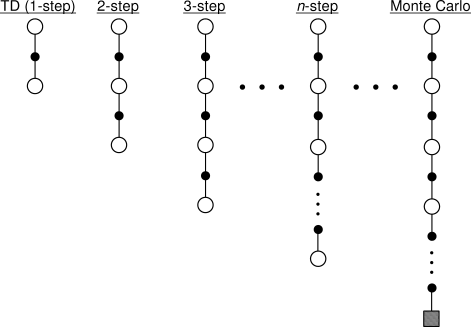
\includegraphics[width=.8\linewidth]{images/nStepTD.png}
\caption[$n$-step returns]{Returns each based on a different amount of rewards and by using the state value as a proxy afterwards. This is not needed for Monte Carlo methods as they use all the future rewards. Source: \cite{Sutton1998ReinforcementIntroduction}.}
\label{fig:nStepTD}
\end{figure}
The $n$-step target can be formulated as:
\begin{equation}
R_t^{(n)} = r_{t+1} + \gamma r_{t+2} + \dots + \gamma^{n-1}r_{t+n} + \gamma^n V_t(s_{t+n})
\end{equation}
There, we treat the terminal state as a state that always transitions to itself with zero reward. This way of treating an episodic task the same as a continuing task doesn't influence the result, even if we discount the returns. As such, all $n$-step returns that last up to or past termination have the same value as the complete return.\\
The increment to $V_t(s_t)$ is then defined by:
\begin{equation}
\Delta V_t(s_t) = \alpha \big[ R_t^{(n)} - V_t(s_t) \big]
\end{equation}
In on-line updating, the updates are done during the episode, as soon as a $\Delta V_t(s_t)$ is computed. In off-line updating, these increments are set aside and applied after the episode is done.\\
$n$-step TD methods are rarely used because they are inconvenient to implement. To compute $n$-step returns, you have to wait $n$ steps to observe the resultant rewards and states.\\

We can also take the weighted average of $n$-step return. This is called the forward view or theoretical view. The requirement is that the weights sum to 1. TD($\lambda$) is a particular way of doing this. The $\lambda$-return is defined by
\begin{equation}
R^\lambda_t = (1-\lambda) \sum_{n=1}^{\infty} \lambda^{n-1} R_t^{(n)}
\end{equation}
After a terminal state has been reached, all subsequent $n$-step returns are equal to $R_t$, so the $(1-\lambda)$ isn't applied. When $\lambda=1$, we will only have the conventional return $R_t$. The increment, $\Delta V_t(s_t)$, is:
\begin{equation}
\Delta V_t(s_t) = \alpha \big[ R_t^{\lambda} - V_t(s_t) \big]
\end{equation}
In this forward view, we look for each state visited forward in time to all the future rewards and decide how best to combine them. After looking forward from and updating one state, we move to the next and don't work with that state anymore. Future states, however, are viewed and processed repeatedly. This way of thinking is visualized in Figure \ref{fig:TDForwardView}.
\begin{figure}[htb]
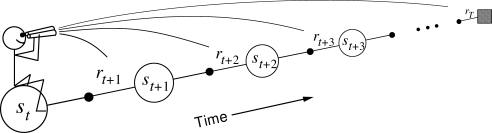
\includegraphics[width=.9\linewidth]{images/TDForwardView.png}
\caption[TD forward view]{The forward view, where each state value is updated by looking forward to the states and their rewards that follow. Source: \cite{Sutton1998ReinforcementIntroduction}.}
\label{fig:TDForwardView}
\end{figure}

The backward view can be seen as a practical version of the forward view, as it achieves the same but is easier to implement.
Here we have an additional memory variable associated with each state, the eligibility trace, denoted $e_t(s) \in \rm I\!R^+$. On each step, they are decayed by $\gamma \lambda$, and the eligibility trace for the one state visited on the step is incremented by 1. The increment $\Delta V_t(s_t)$ is then defined as such:
\begin{subequations}
\label{eq:backview}
\begin{align}
\delta_t &= r_{t+1} + \gamma V_t(s_{t+1}) - V_t(s_t) \label{eq:backview1} \\
\Delta V_t(s) &= \alpha \delta_t e_t(s), \qquad \text{for all} \quad s \in S \label{eq:backview2}
\end{align}
\end{subequations}
Here we work backwards and update backward to each prior state according to the state's eligibility trace at that time. This is visualized in Figure \ref{fig:TDBackwardView}.
\begin{figure}[htb]
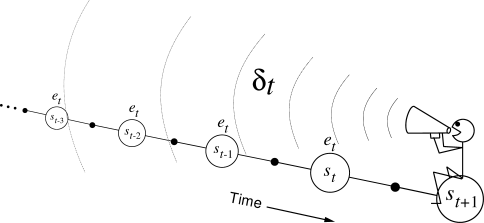
\includegraphics[width=.9\linewidth]{images/TDBackwardView.png}
\caption[TD backward view]{The backward view, where the value of visited states are updated based on their eligibility values. Source: \cite{Sutton1998ReinforcementIntroduction}.}
\label{fig:TDBackwardView}
\end{figure}
If we set $\lambda = 0$, then we only update the trace for $s_t$, thus getting TD(0). For larger values, with $\lambda < 1$, more of the preceding states are changed. The more distant states are changed by a smaller amount because the eligibility trace is smaller. This way, they are blamed less for the TD error.\\
If $\lambda = 1$ the credit given to earlier states falls only by $\gamma$ per step. If $\lambda = 1$ and $\gamma = 1$, then there is no decay at all and we achieve the Monte Carlo method for an undiscounted episodic task. This is known as TD(1). This TD(1) is more general however because it cannot only be applied to episodic tasks, but also to discounted continuing tasks. It can also be performed incrementally and on-line, while Monte Carlo methods have to wait until the episode is over. If the Monte Carlo control method does something bad, its behavior cannot change during the same episode, while on-line TD(1) can (using $n$-step).\\
Both methods achieve the same weight update.\\

To combine TD($\lambda$) and Sarsa, called Sarsa($\lambda$), we need eligibility traces for each state-action pair: $e_t(s,a)$. As such, we do updates like this:
\begin{equation}
Q_{t+1}(s,a) = Q_t(s,a) + \alpha \delta_t e_t(s,a), \qquad \text{for all} \quad s,a
\end{equation}
where
\begin{equation}
\delta_t = r_{t+1} + \gamma Q_t(s_{t+1},a_{t+1}) - Q_t(s_t,a_t)
\end{equation}
and
\begin{equation}
e_t(s,a) = \begin{cases}
    \gamma \lambda e_{t-1}(s,a) + 1 & \text{if $s=s_t$ and $a=a_t$;} \\
    \gamma \lambda e_{t-1}(s,a) & \text{otherwise}.
\end{cases}
\qquad \text{for all $s,a$}
\end{equation}
The resulting algorithm can be seen in Algorithm~\ref{algo:sarsalambda}:\\
\begin{algorithm}[htb]
\DontPrintSemicolon
Initialize $Q(s,a)$ arbitrarily\;
$e(s,a) \gets 0$ for all $s,a$\;
\For{each episode} {
    Initialize s,a\;
    \Repeat{$s$ is terminal} {
        Take action $a$, observe reward $r$ and new state $s'$\;
        Choose action $a'$ from $s'$ with action selection policy using $Q$\;
        $\delta = r + \gamma Q(s',a') - Q_t(s,a)$\;
        $e(s,a) \gets e(s,a) + 1$\;
        \For{all $s,a$} {
            $Q(s,a) \gets Q(s,a) + \alpha \delta e(s,a)$\;
            $e(s,a) \gets \gamma \lambda e(s,a)$\;
        }
        $s \gets s'$; $a \gets a'$\;
    }
}
\caption[Sarsa($\lambda$)]{Sarsa($\lambda$). Source: \cite{Sutton1998ReinforcementIntroduction}}
\label{algo:sarsalambda}
\end{algorithm}
Two methods exist to combine TD($\lambda$) and Q-learning and thus getting Q($\lambda$): There exists 2 different methods: Watkins' Q($\lambda$) and Peng's Q($\lambda$).\\
Here, we must cut off the look ahead until the first exploratory action instead of the episode's end. This is done because this exploratory action doesn't have any relationship with the greedy policy. Recall that Q-learning is an off-policy method and the policy learned about is not necessarily the same as the one used to select actions. As such, it can learn about the greedy policy while following a policy involving exploratory (suboptimal) actions.

For Watkins' Q($\lambda$), if $a_{t+n}$ is the first exploratory action, the longest backup is toward:
\begin{equation}
r_{t+1} + \gamma r_{t+2} + \dots + \gamma^{n-1} r_{t+n} + \gamma^n \max_a Q_t(s_{t+n},a)
\end{equation}
Where we assume off-line updating.\\
In the backward view, we update the eligibility traces just like in Sarsa, with the only exception that we don't use the eligibility trace of the previous time step when a suboptimal (exploratory) action is taken. We get the following result:
\begin{equation}
e_t(s,a) = I_{s s_t} * I_{a a_t} + \begin{cases}
    \gamma \lambda e_{t-1}(s,a) & \text{if $Q_{t-1}(s_t,a_t) = \max_a Q_{t-1}(s_t,a)$;} \\
    0 & \text{otherwise}
\end{cases}
\end{equation}
Where $I_{xy}$ is an identity indicator function, equal to $1$ if $x=y$ and $0$ otherwise. The Q update is defined by:
\begin{equation}
Q_{t+1}(s,a) = Q_t(s,a) + \alpha \delta_t e_t(s,a)
\end{equation}
Where
\begin{equation}
\delta_t = r_{t+1} + \gamma \max_{a'} Q_t(s_{t+1}, a') - Q_t(s_t,a_t)
\end{equation}
The resulting pseudo-code can be seen in Algorithm~\ref{algo:watkinsq}.\\
\begin{algorithm}[htb]
\DontPrintSemicolon
Initialize $Q(s,a)$ arbitrarily\;
$e(s,a) \gets 0$ for all $s,a$\;
\For{each episode} {
    Initialize s,a\;
    \Repeat{$s$ is terminal} {
        Take action $a$, observe reward $r$ and new state $s'$\;
        Choose action $a'$ from $s'$ with action selection policy using $Q$\;
        $a^* \gets \argmax_b Q(s',b)$\;
        \If{$a^* = a'$} {
            $a^* \gets a'$\;
        }
        $\delta = r + \gamma Q(s',a^*) - Q_t(s,a)$\;
        $e(s,a) \gets e(s,a) + 1$\;
        \For{all $s,a$} {
            $Q(s,a) \gets Q(s,a) + \alpha \delta e(s,a)$\;
            \eIf{$a^* = a'$} {
                $e(s,a) \gets \gamma \lambda e(s,a)$\;
            }{
                $e(s,a) \gets 0$\;
            }
        }
        $s \gets s'$; $a \gets a'$\;
    }
}
\caption[Watkins' Q($\lambda$)]{Watkins' Q($\lambda$). Source: \cite{Sutton1998ReinforcementIntroduction}}
\label{algo:watkinsq}
\end{algorithm}
Because exploratory actions happen often, backups won't be long and so eligibility traces won't have a lot of advantage anymore.\\
Peng's Q($\lambda$) tries to solve this, being a hybrid of Sarsa($\lambda$) and Watkin's Q($\lambda$). Its component backups are neither off- nor on-policy. The earlier transitions are each on-policy and the last transition uses the greedy policy. As such, all but the last uses the actual experiences. Because of this, for a fixed non-greedy policy, $Q_t$ converges to neither $Q^{\pi}$ nor $Q^{*}$, but some hybrid between the 2. If the policy is more greedy, the method may still converge to $Q^{*}$.\\

Replacing traces are a modified kind of eligibility traces that can yield a slightly better performance. With the traditional kind of traces (accumulating traces), the trace of a state is augmented by 1 when visiting it. With replacing traces, however, they are set to $1$. Thus, we get the following update:
\begin{equation}
e_t(s) = \begin{cases}
1 & \text{if $s=s_t$}\\
\gamma \lambda e_{t-1}(s) & \text{otherwise}
\end{cases}
\end{equation}
Prediction or control algorithms using this are called replace-trace methods.
\begin{equation}
e_t(s,a) = \begin{cases}
1 + \gamma \lambda e_{t-1}(s,a) & \text{if $s=s_t$ and $a=a_t$;}\\
0 & \text{if $s=s_t$ and $a \neq a_t$;} \qquad \text{for all $s,a$}\\
\gamma \lambda e_{t-1}(s,a) & \text{if $s \neq s_t$.}
\end{cases}
\end{equation}

Another possible improvement if set correctly is a variable $\lambda$, which can be different at each time step $t$. It can for example depend on the current state: $\lambda_t = \lambda(s_t)$. It can be set to zero when we are sure about the estimate of the state $s_t$, so we don't have to use estimates of following states anymore. By setting it to $1$, we can achieve the opposite.

\todo[inline]{Check if next section blends in correctly}
%Off-policy bootstrapping
\section{Bootstrapping}
\label{sec:rl:bootstrapping}
Bootstrapping is the updating of a value estimate based on other value estimates. This is done by TD and DP methods, but not by Monte Carlo methods. TD($\lambda$) is a bootstrapping method when $\lambda <1$, but not when $\lambda = 1$. Although the latter involves bootstrapping within an episode, afterwards the effect over a complete episode is the same as the non-bootstrapping Monte Carlo update. Bootstrapping methods such as TD($\lambda$) are harder to combine with function approximation because they only find near-minimal MSE solutions (only for the on-policy distribution) instead of the minimal MSE using for example linear, gradient-descent function approximation for any distribution of training examples, $P$.\\
The restriction of convergence is especially a problem for off-policy methods such as Q-learning and DP methods because they do not backup states (or state-action pairs) with exactly the same distribution as the distribution of states we encounter when following the policy of which we want to estimate the value function. Off-policy bootstrapping combined with function approximation can even lead to divergence and infinite MSE.\\

Bootstrapping looks like a bad idea because non-bootstrapping methods are more easy and reliably used with function approximation and can be applied over a broader range of conditions.
Non-bootstrapping methods also achieve a lower error in approaching the value function, even when backups are done according to the on-policy distribution \parencite{ML}.
In practice, however, bootstrapping methods achieve better performance. When $\lambda$ approaches $1$, which is the non-bootstrapping case, the performance becomes much worse.

\section{Policy gradient}
\label{sub:rl:policy_gradient}
%By David Silver.\\

Here, we parametrize the policy instead of the state value or state-action value function.
Methods that parametrize the policy tend to have better convergence properties \parencite{Sutton1999PolicyApproximation}.
No value must be stored for every specific state and action. This is useful in problems where the state and/or action space is high-dimensional and/or continuous. Last, they can also learn policies where a probability is provided for every action.
However, policy gradient methods also come with a few disadvantages. They typically converge to a local optimum instead of a global optimum. It is also rather hard to evaluate a policy and it can have a high variance.\\
The policy gradient has the form of $\pi_{\theta}(s,a)$. The way of measuring the quality of a policy (i.e.\ how well it performs in an environment) depends on the type of environment:
\begin{itemize}
\item Episodic environments: use the value of the start state:
        \begin{equation}
            J_1(\theta) = V^{\pi_{\theta}}(s_1) = \ex_{\pi_{\theta}} [v_1]
        \end{equation}
\item Continuing environments: use the average value:
        \begin{equation}
            J_{avV}(\theta) = \sum_s d^{\pi_{\theta}}(s)V^{\pi_{\theta}}(s)
        \end{equation}
\item or the average reward per time step:
        \begin{equation}
            J_{avR}(\theta) = \sum_s d^{\pi_{\theta}} \sum_a \pi_{\theta}(s,a) R_s^a
        \end{equation}
\end{itemize}
Where $d^{\pi_{\theta}}$ is the stationary distribution of the Markov chain for $\pi_{\theta}$. The stationary distribution $\bar{\pi}$ of a Markov distribution $P$ is a probability distribution such that $\bar{\pi} = \bar{\pi} P$. It can be thought of as denoting how much time is spent in each state. This way, values/rewards of states which are visited often are given a higher importance.\\
As such, we need to find the parameters $\theta$ that maximize $J(\theta)$. This optimization problem can be solved using approaches that don't use a gradient, such as hill climbing or genetic algorithms. However, here we focus on gradient descent. In this case, we move the parameter values along the gradient using the quality function: $\Delta \theta = \alpha \nabla_{\theta} J(\theta)$, where $\alpha$ is the step-size parameter and $\nabla_{\theta} J(\theta)$ is the partial derivative for every dimension of $\theta$. To estimate each partial derivative, we can compute the policy objective function $J(\theta)$ for a slightly changed value of $\theta$, determined by $\epsilon$. For each dimension $k$, this is:
\begin{equation}
\frac{\partial J(\theta)}{\partial \theta_k} \approx \frac{J(\theta + \epsilon u_k) - J(\theta)}{\epsilon}
\end{equation}
where $u_k$ is a one-hot vector with a value of $1$ in dimension $k$ and $0$ elsewhere. This kind of gradient is called a Finite Difference gradient. It is a simple, black-box way that works for every policy (because we don't need the derivative), but it is inaccurate and inefficient. We also need to determine the value of $\epsilon$ ourselves, which influences the accuracy.\\

Instead, we will solve the problem analytically. We assume that the policy is differentiable when it is non-zero and that we know the gradient.

%What is likelihood?
% Likelihood is a funny concept. It’s not a probability, but it is proportional to a probability. The likelihood of a hypothesis (H) given some data (D) is proportional to the probability of obtaining D given that H is true, multiplied by an arbitrary positive constant (K). In other words, L(H|D) = K · P(D|H). Since a likelihood isn’t actually a probability it doesn’t obey various rules of probability. For example, likelihood need not sum to 1.

% A critical difference between probability and likelihood is in the interpretation of what is fixed and what can vary. In the case of a conditional probability, P(D|H), the hypothesis is fixed and the data are free to vary. Likelihood, however, is the opposite. The likelihood of a hypothesis, L(H|D), conditions on the data as if they are fixed while allowing the hypotheses to vary.

% The distinction is subtle, so I’ll say it again. For conditional probability, the hypothesis is treated as a given and the data are free to vary. For likelihood, the data are a given and the hypotheses vary.
% Source (with more explanation): https://alexanderetz.com/2015/04/15/understanding-bayes-a-look-at-the-likelihood/
% \todo{TODO: Explain likelihood?}
Likelihood ratios use the following identity:
\begin{align}
\begin{split}
\nabla_{\theta}\pi_{\theta}(s,a) &= \pi_{\theta}(s,a) \frac{\nabla_{\theta}\pi_{\theta}(s,a)}{\pi_{\theta}(s,a)}\\
&= \pi_{\theta}(s,a) \nabla_{\theta} \log \pi_{\theta}(s,a)
\end{split}
\end{align}
Writing it using the $\log$ is possible because $(\log f)' = \frac{f'}{f}$. The score function is $\nabla_{\theta} \log \pi_{\theta}(s,a)$.\\
This can now be used with for example a softmax policy. Here, we weight actions using a linear combination of features: $\phi(s_a)^T \theta$. The probability of an action is then the following proportion:
\begin{equation}
\pi_{\theta}(s,a) \propto \rm{e}^{\phi(s,a)^T \theta}
\end{equation}
The score function is here defined as being:
\begin{equation}
\nabla_{\theta} \log \pi_{\theta}(s,a) = \phi(s,a) - \ex_{\pi_{\theta}}[\phi(s,\cdot)]
\end{equation}
When having a continuous action space, it is better to use a Gaussian policy, where the mean is a linear combination $\mu(s) = \phi(s)^T \theta$ and the variance can be either fixed or also parametrized. The policy is then $a \sim N(\mu(s), \sigma^2)$. The score function here is defined as being:
\begin{equation}
\nabla_{\theta} \log \pi_{\theta}(s,a) = \frac{(a-\mu(s))\phi(s)}{\sigma^2}
\end{equation}
We can now use the likelihood ratios to compute the policy gradients for one-step Markov decision processes:
\begin{subequations}
\begin{align}
\begin{split}
J(\theta) &= \ex_{\pi_{\theta}}[r]\\
&= \sum_{s \in S} d(s) \sum_{a \in A} \pi_{\theta}(s,a) R(s,a)
\end{split}\\
\begin{split}
\nabla_{\theta} J(\theta) &= \sum_{s \in S} d(s) \sum_{a \in A} \pi_{\theta}(s,a) \nabla_{\theta} \log \pi_{\theta}(s,a) R(s,a)\\
&= \ex_{\pi_{\theta}} [\nabla_{\theta} \log \pi_{\theta}(s,a)r]
\end{split}
\end{align}
\end{subequations}
%Got it from here: https://pdfs.semanticscholar.org/eb5b/459c8a3e56064158fb3514eeab763486e437.pdf but I interpreted it wrong. However, REINFORCE may do something like , by averaging these gradients over multiple trajectories. So it may be useful to look into it
% \todo{Next part is wrong, see comment}
% When considering multiple trajectories $\tau \sim p_\theta(\tau) = p(\tau \vert \theta)$, we can compute the quality like this:
% \begin{equation}
% J(\theta) = \int_{T} p_{\theta}(\tau \vert \pi)r(\tau) d\tau
% \end{equation}
% Where $r(\tau) = \sum_{k=0} \gamma^k r_k$. We again have a gradient:
% \begin{equation}
% \nabla_{\theta}J_{\theta} = \nabla_{\theta} \int_{T} p_{\theta}(\tau \vert \pi)r(\tau) d\tau = \int_T \nabla_{\theta} p_{\theta}(\tau \vert \pi) r(\tau) d\tau
% \end{equation}
% Using again the $\log$ trick, we get:
% \begin{align}
% \nabla_{\theta}J(\theta) &= \int_T p_{\theta}(\tau \vert \pi) \nabla \log p_{\theta} (\tau \vert \pi) r(\tau) d\tau\\
% &= E[\nabla_{\theta} \log p_{\theta}(\tau \vert \pi)r(\tau)]\\
% &\approx \frac{1}{K} \sum_{k=1}^K \nabla_{\theta} \log p_{\theta}(\tau \vert \pi) r(\tau_k)
% \end{align}
The Policy Gradient theorem states that we can use this for multi-step MDP's \parencite{Sutton1999PolicyApproximation}. We can do this by replacing the reward with the state-action value:
\begin{equation}
\ex_{\pi_{\theta}} [\nabla_{\theta} \log \pi_{\theta}(s,a)Q^{\pi_{\theta}}(s,a)]
\end{equation}
Monte-Carlo policy gradients use this policy gradient theorem and update parameters using stochastic gradient descent. For this, a return $v_t$ is used as an unbiased sample of $Q^{\pi_{\theta}}(s,a)$. The resulting algorithm is called \textit{REINFORCE} \parencite{williams1992simple} and is shown in Algorithm~\ref{algo:reinforce}.\\
\begin{algorithm}[htb]
\DontPrintSemicolon
Initialize $\theta$ arbitrarily\;
\For{each episode $\{s_1, a_1, r_2, \dots, s_{T_1}, a_{T_1}, r_T\} \sim \pi_{\theta}$} {
    \For{$t=1$ to $T-1$} {
        $\theta \gets \theta + \alpha \nabla_{\theta} \log \pi_{\theta}(s_t,a_t)v_t$
    }
}
\Return $\theta$
\caption[REINFORCE]{REINFORCE algorithm. Source: \cite{Sutton1998ReinforcementIntroduction}.}
\label{algo:reinforce}
\end{algorithm}

The problem with the Monte-Carlo policy gradient is that it has a high variance. This can be solved by using an actor-critic method. The critic is used to update the state-action value function parameters $w$, such that $Q_w(s,a) \approx Q^{\pi_{\theta}}(s,a)$, while the actor updates the policy parameters $\theta$ in the direction suggested by the critic. These actor-critic algorithms follow an approximate policy gradient:
\begin{align}
\nabla_{\theta}J(\theta) &\approx \ex_{\pi_{\theta}}[\nabla_{\theta} \log \pi_{\theta}(s,a) Q_w(s,a)]\\
\Delta \theta &= \alpha \nabla_{\theta} \log \pi_{\theta}(s,a) Q_w(s,a)
\end{align}
The critic function can be seen of a way of evaluating how good the policy is for the current $\theta$. A simple way of computing $Q_w(s,a)$ is simply a linear function of $w$ and $\phi(s,a)$: $Q_w(s,a) = \phi(s,a)^T w$. The algorithm, named \textit{QAC} is shown in Algorithm~\ref{algo:qac}.\\
\begin{algorithm}[htb]
\DontPrintSemicolon
Initialize $s,\theta$\;
Sample $a \sim \pi_{\theta}$\;
\For{each step} {
    Sample reward $r = R_s^a$; sample transition $s' \sim P_s^a$\;
    Sample action $a' \sim \pi_{\theta}(s',a')$\;
    $\delta = r + \gamma Q_w(s',a') - Q_w(s,a)$\;
    $\theta = \theta + \alpha \nabla_{\theta} \log \pi_{\theta}(s,a)Q_w(s,a)$\;
    $w \gets w + \beta \delta \phi (s,a)$\;
    $a \gets a'$, $s \gets s'$\;
    }
\caption{QAC}
\label{algo:qac}
\end{algorithm}
For a function approximation to be compatible, it needs to fulfill 2 conditions:
\begin{itemize}
\item The value function approximator is compatible to the policy: $\nabla_w Q_w(s,a) = \nabla_{\theta} \log \pi_{\theta}(s,a)$
\item The value function parameters w minimize the mean-squared error: $\epsilon = \ex_{\pi_{\theta}} [(Q^{\pi_{\theta}}(s,a) - Q_w(s,a))^2]$
\end{itemize}
The policy gradient will then be exactly:
\begin{equation}
\nabla_{\theta}J(\theta) = \ex_{\pi_{\theta}} [\nabla_{\theta} \log \pi_{\theta}(s,a) Q_w(s,a)]
\end{equation}
To reduce the variance in the policy gradient we subtract the baseline function $B(s)$ from it. This doesn't change the expectation:
\begin{align}
\begin{split}
\ex_{\pi_{\theta}} [\nabla_{\theta} \log \pi_{\theta}(s,a)B(s)] &= \sum_{s \in S} d^{\pi_{\theta}}(s) \sum_a \nabla_{\theta} \pi_{\theta}(s,a)B(s)\\
&= \sum_{s \in S} d^{\pi_{\theta}}B(s)\nabla_{\theta} \sum_{a \in A} \pi_{\theta} (s,a)\\
&= 0
\end{split}
\end{align}
A good baseline function is the state value function: $B(s) = V^{\pi_{\theta}}$. When this is used as a baseline function, we can rewrite the policy gradient using the advantage function $A^{\pi_{\theta}}(s,a)$:
\begin{align}
A^{\pi_{\theta}}(s,a) &= Q^{\pi_{\theta}}(s,a) - V^{\pi_{\theta}}(s)\\
\nabla_{\theta}J(\theta) &= \ex_{\pi_{\theta}}[\nabla_{\theta} \log \pi_{\theta}(s,a) A^{\pi_{\theta}}(s,a)]
\end{align}
This still reduces the variance. The critic should now estimate the advantage function. This can be done by estimating both $V^{\pi_{\theta}}(s)$ and $Q^{\pi_{\theta}}(s,a)$. With those 2 function approximators we then get:
\begin{align}
V_v(s) &\approx V^{\pi_{\theta}}(s)\\
Q_w(s,a) &\approx Q^{\pi_{\theta}}(s,a)\\
A(s,a) &= Q_w(s,a) - V_v(s)
\end{align}
For updating those values, we can again use temporal difference learning. The TD error is:
\begin{equation}
\delta^{\pi_{\theta}} = r + \gamma V^{\pi_{\theta}}(s') - V^{\pi_{\theta}}(s)
\end{equation}
This is an unbiased estimate of the advantage function:
\begin{align}
\begin{split}
\ex_{\pi_{\theta}}[\delta^{\pi_{\theta}} | s,a] &= \ex_{\pi_{\theta}}[r + \gamma V^{\pi_{\theta}}(s') | s,a] - V^{\pi_{\theta}}(s)\\
&= Q^{\pi_{\theta}}(s,a) - V^{\pi_{\theta}}(s)\\
&= A^{\pi_{\theta}}(s,a)
\end{split}
\end{align}
As such, we can use this TD error to compute the policy gradient:
\begin{equation}
\nabla_{\theta}J(\theta) = \ex_{\pi_{\theta}}[\nabla_{\theta} \log \pi_{\theta}(s,a) \delta^{\pi_{\theta}}]
\end{equation}
In practice, we use the function approximator of the critic function for the value function, using the critic parameters $v$:
\begin{equation}
\delta_v = r + \gamma V_v(s') - V_v(s)
\end{equation}

%Chapter 8
\section{Generalization and function approximation}
\label{sub:rl:gfa}
Normally, if there are a lot of possible states, it will take a long time to learn the estimates of all states. It is even possible that, after some time, previously unseen states will be encountered. This problem is possible when using continuous variables, images, \dots To solve this, we generalize states. As such, we can apply information of seen states to related states that haven't been visited yet. To do this, we combine standard reinforcement learning methods with generalization methods.\\

A well known kind of generalization methods is called function approximation: it takes examples of a desired function and tries to approximate it. This is supervised learning (the input is the original value and the output to predict is the generalized value). The used supervised learning algorithm needs to be able to handle non-stationary target functions, as learning must be able to occur on-line. The error for the algorithm to minimize is the mean-squared error (MSE) between the true value of the state and the approximated one:
\begin{equation}
MSE(\overrightarrow{\theta_t}) = \sum_{s \in S} P(s) \big[ V^{\pi}(s) - V_t(s) \big]^2
\end{equation}
Where $\theta_t$ is a component of the model that the algorithm generated and $P$ is a distribution weighting the errors of different states. As there are less components $\overrightarrow{\theta_t}$ than states, the flexibility for approximation is limited. Because of this, we use $P$ to define the trade-offs of focusing on improving the approximation of some states at the expense of others. Usually, this distribution $P$ is the same as the one from which the states in the training examples are drawn from and thus the distribution of states at which backups are done. For minimizing the error over a certain distribution of states, it is of course preferred that the training examples come from the same distribution.\\
Another interesting distribution is the on-policy distribution, which describes the frequency with which states are encountered while the agent is interacting with the environment and selecting actions according to policy $\pi$. Minimizing the error over this distribution, we concentrate on states that actually occur while following the policy and ignoring others. Training examples for this distribution are also the easiest to get using Monte Carlo or TD methods because they generate backups from sample experience using the policy $\pi$.\\
%Minimizing the MSE may not lead to finding the best predictions. However, we have no alternative yet.\\
For simple function approximators such as linear ones, the best MSE we find might also be the global optimum. This is however rarely possible for more complex ones, e.g.\ kernel based methods or artificial neural networks, and they may stop at a local optimum. For many cases of interest in reinforcement learning, convergence to an optimum, i.e.\ achieving the highest possible reward, does not occur.\\

One of the most widely used function approximation methods is based on gradient descent. Here, the parameter vector is a column vector with a fixed number of real valued components, also called a weight vector: $\overrightarrow{\theta_t} = (\theta_t(1), \theta_t(2), \dots, \theta_t(n)^T$. $V_t(s)$ is a smooth differentiable function of $\overrightarrow{\theta_t}$ for all $s \in S$.
At each time step $t$, we observe a new example $s_t \mapsto V^{\pi}(s_t)$.
The order of the received states is not assumed to be the same as the order of gathering them from transitions in the environment.
Even if we would give the exact $V^{\pi}(s_t)$, the function approximator has only limited resources and would not be able to approximate the function exactly. Thus, it must generalize.\\
Like already discussed, we assume that the states over which we want to minimize the MSE over come from the same distribution $P$ as the from examples.
We can then use gradient descent, explained in Section~\ref{ssub:gradient_descent}, to adjust the parameter vector in order to minimize the error:
\begin{align}
\begin{split}
\overrightarrow{\theta}_{t+1} &= \overrightarrow{\theta}_t - \frac{1}{2} \alpha \Delta_{\overrightarrow{\theta}_t} \big[ V^{\pi}(s_t) - V_t(s_t) \big]^2\\
&= \overrightarrow{\theta}_t + \alpha \big[ V^{\pi}(s_t) - V_t(s_t) \big] \Delta_{\overrightarrow{\theta}_t} V_t(s_t)
\end{split}
\end{align}
Where $\alpha$ is a positive step-size parameter and $\nabla_{\overrightarrow{\theta}_t}$ denotes the vector of partial derivatives for every function $f$.\\
If $V^{\pi}(s_t)$ is unavailable because we only have a noise-corrupted version or one with backed-up values, we can simple use $v_t$ instead of $V^{\pi}(s_t)$:
\begin{equation}
\overrightarrow{\theta}_{t+1} = \overrightarrow{\theta}_t + \alpha \big[ v_t - V_t(s_t) \big] \Delta_{\overrightarrow{\theta}_t} V_t(s_t)
\end{equation}
If $v_t$ is an unbiased estimate and so $E\{v_t\} = V^{\pi}(s_t)$ for each $t$, then $\overrightarrow{\theta}_t$ is guaranteed to converge to a local optimum under stochastic approximation conditions for decreasing the step-size parameter $\alpha$. This is the case for Monte Carlo state-value prediction.\\

An important special case is when the approximate function $V_t$ is a linear function of the parameter vector, $\overrightarrow{\theta}_t$. For every state $s$, there is a column vector of features $\overrightarrow{\phi}_s = (\phi_s(1), \phi_s(2), \dots, \phi_s(n))^T$, with the same number of components as $\overrightarrow{\theta}_t$. The approximate state-value function is then given by:
\begin{equation}
V_t(s) = \overrightarrow{\theta}_t^T \overrightarrow{\phi}_s = \sum_{i=1}^n \theta_t(i) \phi_s(i)
\end{equation}
The gradient with respect to $\overrightarrow{\theta}_t$ is then:
\begin{equation}
\nabla_{\overrightarrow{\theta}_t} V_t(s) = \overrightarrow{\phi}_s
\end{equation}
As can be seen, this update is rather simple. Furthermore, there is only one optimum (or several ones which are equally good), $\overrightarrow{\theta}^{*}$. As a result, the method is guaranteed to converge to or near a local optimum.\\
Note that this linear form doesn't allow for the representation of interactions between features, for example when the presence of a certain features is good only if another feature is absent. For this, we need to introduce features that are combinations of feature values.\\

\subsection{Coarse coding}
\label{subs:rl_cc}
Coarse coding is the representation of a state with features that overlap, for example a binary feature that is $1$ when the coordinate given by a $x$ and $y$ feature lies in a circle. If 2 points \textit{A} and \textit{B} have circles "in common", there will be some generalization between them, as the features for both points for those circles will be 1. This is shown in Figure~\ref{fig:coarsecoding1}. The more features in common, the greater this effect.
\begin{figure}[htb]
\captionsetup{width=0.8\textwidth}
\centering
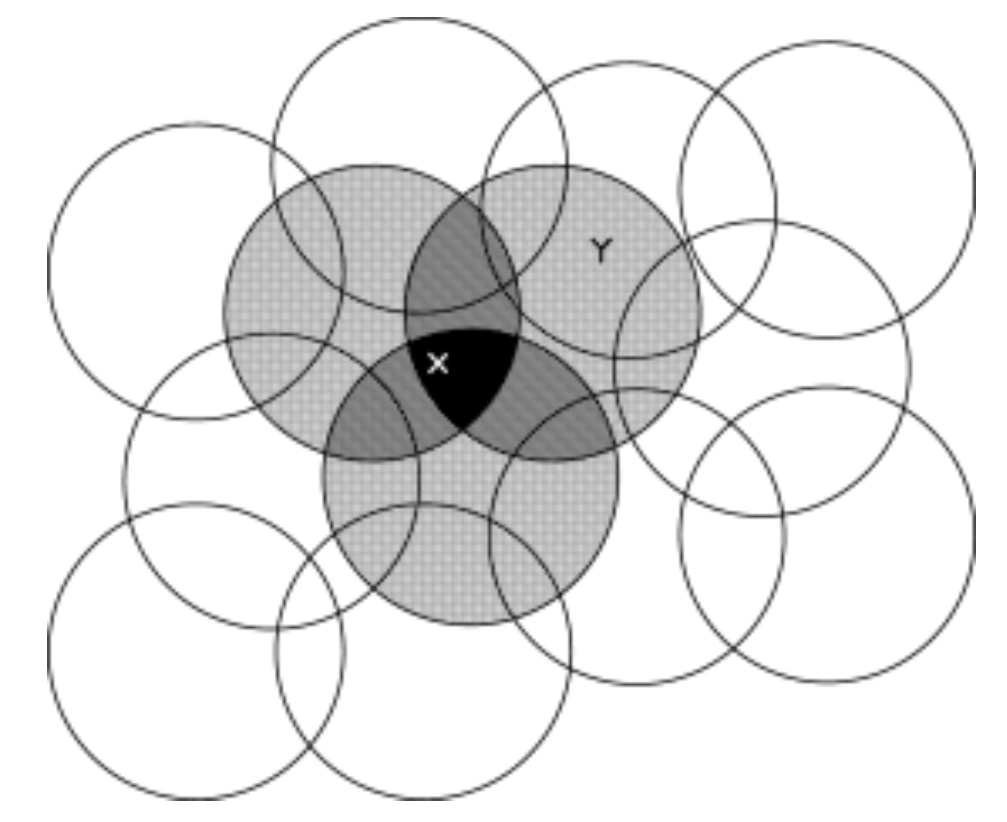
\includegraphics[width=0.5\linewidth]{images/coarsecoding1.png}
\caption[Generalization between points]{$X$ and $Y$ share 1 feature, as both points lie in the same receptive field, a circle. Thus, slight generalization from $X$ to $Y$ is possible. Source: \cite{Sutton1998ReinforcementIntroduction}.}
\label{fig:coarsecoding1}
\end{figure}
If the circles are small or large, generalization will be over respectively a short or large distance. The nature of the generalization is also affected by the shape of the features' receptive fields.  This can be seen in Figure~\ref{fig:coarsecoding2}. The fineness of discrimination is however only determined by the total number of features.
\begin{figure}[htb]
\captionsetup{width=0.8\textwidth}
\centering
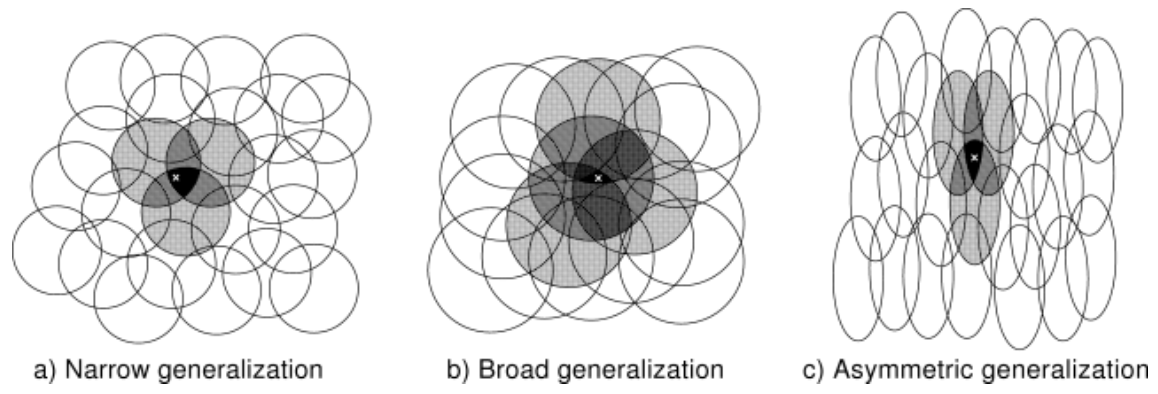
\includegraphics[width=0.8\linewidth]{images/coarsecoding2.png}
\caption[Shapes of receptive fields]{Generalization depends on the shape of the receptive fields of the features. When multiple features' receptive fields overlap, the generalization is broad and narrow when only few of them overlap. Source: \cite{Sutton1998ReinforcementIntroduction}.}
\label{fig:coarsecoding2}
\end{figure}

In tile encoding, a form of coarse encoding, the fields of the features are grouped into exhaustive partitions of the input space, called tilings. These tilings are defined by ranges of values for state attributes that they cover. For one specific tiling, the state can only lie in the ranges of 1 tile. As such, maximally one feature is active in each tiling and the total number of features present is always the same as the number of tilings. This allows us to set the step-size parameter $\alpha$ (used in formula \ref{eq:backview1}) in an easy, intuitive way. We can for example choose $\alpha = \frac{1}{m}$, where $m$ is the number of tilings. This results in exact one-trial learning. When the example $s_t \mapsto v_t$ is received, then the new value will be $V_{t+1}(s_t) = v_t$, whatever the prior value $V_t(s_t)$ was. For a slower change using for example $\alpha=\frac{1}{10m}$, one would move one-tenth of the way to the target in one update.\\
The weighted sum to make up the approximate value function is almost trivial to compute, as in tile coding only binary features are used. Instead of performing $n$ multiplications and additions, we compute the indices of the $m<<n$ present features and then add up the $m$ corresponding components of the parameter vector. The eligibility trace computation is also easier because the components of the gradient $\nabla_{\overrightarrow{\theta}} V_t(s_t)$ are either $0$ or $1$.\\
An easy to compute form of tilings are grid-like ones. Different tilings may also be used, ideally offset by different amounts. The width and shapes should match the width of generalization that is expected to be optimal. The denser the tiling, the more fine-grained the desired function can be, but also the greater the computational cost of updating. The width or shape of each tile must not be uniform or regular-shaped (like a square) however. One can also use stripes, diamond shapes, \dots To reduce memory requirements, hashing can be used. A large tiling can be collapsed in such way into a much smaller set of tiles. This hashing produces tiles consisting of non-contiguous, disjoint regions randomly spread throughout the state space, but that still form an exhaustive tiling.\\
Radial basis functions are a generalization of coarse coding that allows for continuous-valued features: in the interval $[0,1]$ instead of just $0$ or $1$. This way, we can reflect various degrees to which the feature is present. A typical RBF feature, $i$, has a Gaussian (bell-shaped) response $\phi_s(i)$ dependent only on the distance between the state and the feature's center state, $c_i$ and relative to the feature's width $\sigma_i$:
\begin{equation}
\phi_s(i) = e^{-\frac{||s-c_i||^2}{2 \sigma^2_i}}
\end{equation}
The advantage of this method is that they produce approximate functions that vary smoothly and are differentiable. The disadvantage is that $\sigma_i$ and $c_i$ must be tuned manually and that non-linear RBF networks are computationally complex.\\
